\section{Обзор}
\subsection{Синтаксический анализ графов}
При работе с графами, например в графовых базах данных, возникает необходимость выполнения запросов поиска путей, удовлетворяющих заданным ограничениям. Ограничения задаются, как правило, регулярной грамматикой, однако контекстно-свободные грамматики представляют собой более выразительный язык запросов. Контекстно-свободная грамматика (КС-грамматика) $G$ --- четверка $(T, N, P, S)$, где $N$ --- множество нетерминалов, $T$ --- множество терминалов ($T \cap N = \varnothing$), $P = \{ A \rightarrow \alpha \mid A \in N, \alpha \in (N \cup T)^*\}$ --- множество правил грамматики и $S \in N$ --- стартовый символ. Грамматика $G = (\{+, -, a\}, \{ E, N \}, P, E)$, множество правил которой $P$ представлены на листинге~\ref{grmG1}, задает язык арифметических выражений со сложением и умножением над переменными $a$.

\begin{listing}
\caption{Правила грамматики $G$}
\label{grmG1}
\centering
$\begin{array}{ll}
E \rightarrow & N \ + \ N \mid N \ - \ N
\\
N \rightarrow & a
\end{array}$
 \end{listing}

Итак, задача выполнения запросов является задачей поиска в ориентированном графе всех путей, представляющих собой строки языка, заданные КС-грамматикой. Одно из возможных решений такой задачи --- это модификация алгоритмов классического синтаксического анализа строк. Работа~\cite{Sevon} модифицирует алгоритм Эрли. Данный подход позволяет записывать запросы к графовым структурам данных с указанием направления поиска: прямое направление, когда поиск производится в направлении ребер графа, или обратном --- по обратным ребрам. Данный алгоритм строит только некоторое приближение к результату: обработка циклов входного графа осуществляется только до некоторой глубины, специфицируемой пользователем, в результате чего некоторые пути могут быть утеряны. Результатом работы алгоритма является подграф, содержащий пути разбора. 

Для последующего анализа путей из результата удобно иметь информацию об их синтаксической структуре, например в форме абстрактных синтаксических деревьев. Так как множество путей может быть бесконечным, то и синтаксических деревьев может быть бесконечно много, поэтому возникает вопрос об их представлении. В алгоритмах обобщенного синтаксического анализа, в случае существования нескольких деревьев разбора для одной строки (в виду неоднозначностей грамматики), используется компактное представление леса разбора SPPF (Shared Packed Parse Forest). В структуре SPPF переиспользуются общие фрагменты разных выводов, за счет его размер полиномиален от размера входной строки. Существуют модификации обобщенных алгоритмов, применимые для выполнения запросов в контекстно-свободных ограничениях к графам: алгоритмы на основе RNGLR~\cite{RNGLR} и GLL~\cite{GrigRagCFPQuerying}. Первый позволяет построить лес разбора SPPF, второй --- бинаризованный лес разбора Binarized Shared Packed Parse Forest~\cite{SPPF} с лучшими пространственными характеристиками. 

Binarized Shared Packed Parse Forest имеет размер $O(n^3)$, где n --- длина входной строки. В отличие от обычного дерева разбора, внутренние узлы которого всегда соответствуют нетерминалам грамматик, в BSPPF используются дополнительные типы узлов: упакованный узел (packed node) и промежуточный узел (intermediate node). Упакованный узел создаётся для представления неоднозначностей вывода (его дети соответствуют разным продукциям). Промежуточный узел используется для бинаризации, когда правило длины больше 2 представляется как цепочка применений правил длины 2. Именно за счет бинаризации достигается кубический размер представления леса разбора. В SPPF могут быть циклы. На рис.~\ref{fig:sppfV} представлено, как выглядит SPPF, состоящее из деревьев на рис.~\ref{fig:sppfA} и рис.~\ref{fig:sppfB}. А на рис.~\ref{fig:sppfG} представлена его бинаризованная форма. Пример взят из статьи~\cite{IzmCombinator}.

 \begin{figure}[t]
 \centering
    \subfloat[Дерево разбора 1]{
        \label{fig:sppfA}
        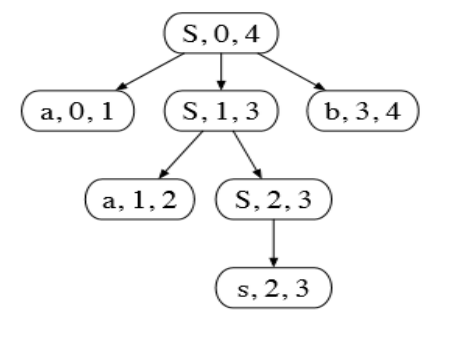
\includegraphics[width=0.35\textwidth]{Smolina/pics/SppfA.png}
    }
    \subfloat[Дерево разбора 2]{
        \label{fig:sppfB}
        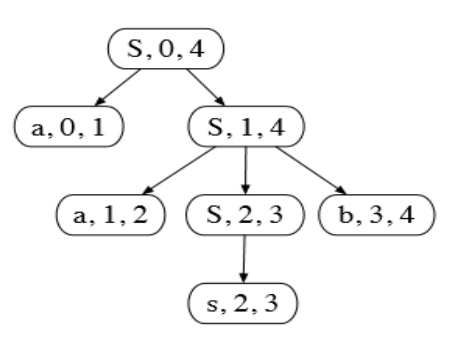
\includegraphics[width=0.35\textwidth]{Smolina/pics/SppfB.png}        
    }

    ~\\~
    \subfloat[SPPF]{
        \label{fig:sppfV}
        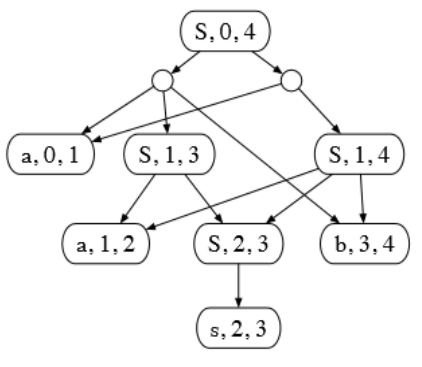
\includegraphics[width=0.35\textwidth]{Smolina/pics/SppfV.png}        
    }
    \subfloat[Бинаризинное SPPF]{
        \label{fig:sppfG}
        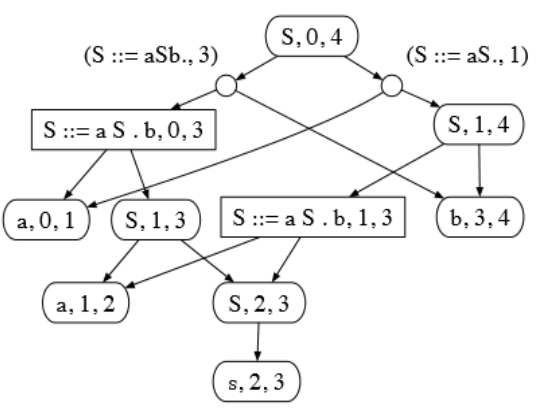
\includegraphics[width=0.45\textwidth]{Smolina/pics/SppfG.png}        
    }
 \caption{Граф SPPF для двух вариантов вывода}
\end{figure}

Решение на RNGLR и GLL построено на основе генерации синтаксических анализаторов. Такое решение не является удобным при работе с графами и графовыми базами данных, так как при добавлении малейших изменений необходимо генерировать руками новый синтаксический анализатор, а также требуется использование дополнительного предметно-ориентированного языка для задания запроса. 

В сфере промышленных графовых баз данных существуют свои языки запросов. К примеру для графовой базы данных Neo4j~\cite{Neo4j} существуют языки Cypher~\cite{Cypher} и openCypher~\cite{openCypher}, а для OrientDB~\cite{OrientDB} используется язык SQL~\cite{Sql}. Ни один из них не поддерживает формат запроса в виде контекстно-свободной грамматики. Более того, результат запроса всегда --- простые строки, что усложняет их дальнейший анализ.

Таким образом, нашей целью стала разработка решения, в котором грамматику можно специфицировать в коде целевого приложения. Один из возможных подходов к решению данной задачи --- использование техники парсер-комбинаторов~\cite{HOFunParsing}.

\subsection{Техника парсер-комбинаторов}
Комбинатор --- это функция высшего порядка, которая из набора функций строит новую функцию. Возможность принимать функции как аргументы, комбинировать их и возвращать как результат является важной особенностью функциональных языков программирования. Парсер-комбинатор --- это функция высшего порядка, которая на вход получает множество синтаксических анализаторов и возвращает новый синтаксический анализатор. 

Для синтаксического анализа необходимо научиться анализировать элементарные сущности (терминалы, нетерминалы), осуществлять последовательное применение анализаторов и поддержать возможность осуществлять выбор анализатора для разбора суффикса сроки. Эти требования задают минимальный набор комбинаторов. Техника парсер-комбинаторов позволяет из элементарных анализаторов конструировать более сложные. Интеграция с языком программирования приложения, в котором применяется синтаксический анализатор, добавляет гибкости и расширяемости в сравнении с генераторами синтаксических анализаторов. Приведём пример реализации простейшего парсер-комбинатора на Scala.

В листинге~\ref{parser1} представлен синтаксический анализатор, который принимает на вход строковую последовательность, затем разбирает строку, начинающуюся с определенного терминала, и возвращает результат разбора и необработанный суффикс строки.

\begin{listing}
\caption{Синтаксический анализатор терминала}
\label{parser1}
\centering
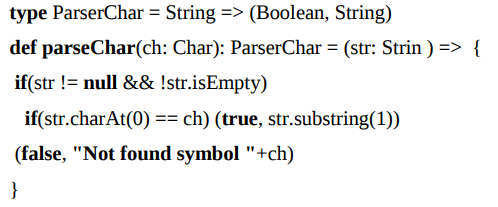
\includegraphics[width=0.7\textwidth]{Smolina/pics/parser1.png}
\end{listing}

Для того чтобы получить синтаксический анализатор подстроки, можно воспользоваться парсер-комбинатором,
который составлял последовательность из анализаторов символов --- парсер-комбинатор последовательности seq. На листинге~\ref{parserSeq} приведен пример реализации.

\begin{listing}
\caption{Парсер-комбинатор последовательности}
\label{parserSeq}
\centering
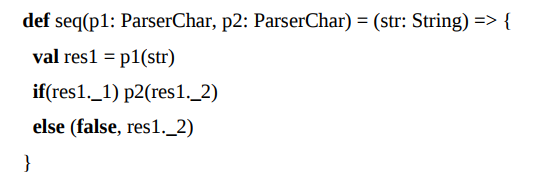
\includegraphics[width=0.7\textwidth]{Smolina/pics/parserSeq.png}
\end{listing}

Теперь, чтобы получить синтаксический анализатор, начинающийся с подстроки ``ABC'', мы можем воспользоваться элементарными синтаксическими анализаторами символов и парсер-комбинатором последовательности (см. листиниг~\ref{parserABC}).

\begin{listing}
\caption{Парсер-комбинатор строки “ABC”}
\label{parserABC}
\centering
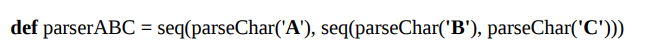
\includegraphics[width=0.9\textwidth]{Smolina/pics/parserABC.png}
\end{listing}

Простые парсер-комбинаторы, основанные на рекурсивном спуске, представляют собой интуитивно ясную модель и поэтому удобны для
отладки. Однако они имеют экспоненциальную сложность относительно размеров грамматики~\cite{Popov}. Это связано с тем, что в наивной реализации рекурсивного спуска при откате не сохраняются результаты и разбор префикса строки одним и тем же синтаксическим анализатором может происходить многократно. Мемоизация~\cite{Memoization} позволяет решить эту проблему за счет переиспользования результатов применения синтаксических анализаторов к подстрокам. Таким образом, однажды выполненное вычисление никогда не повторяется --- результат просто берется из таблицы.

Другой проблемой, ассоциируемой с парсер-комбинаторами, является трудность обработки леворекурсивных определений анализаторов. Например, синтаксический анализ наивным рекурсивным спуском в соответствии с грамматикой, представленной в листинге~\ref{grmG2}, никогда не завершится.

 \begin{listing}
\caption{Леворекурсивная грамматика}
\label{grmG2}
\centering
$\begin{array}{rl}
E \rightarrow E \ + \ a \ | \ a
\end{array}$
 \end{listing}

Данная проблема имеет несколько решений, одно из которых основано на ограничении числа вызовов нетерминала некоторой константой, связанной с длиной входной последовательности ~\cite{ParserComb}. Количество применений каждого распознавателя к каждой позиции в строке ограничивается длиной неразобранного суффикса строки. Данный подход не применим, если длина последовательности неизвестна, например, при считывании символов с сетевого сокета. Во-вторых, такой подход обладает сложностью $O(n^4)$, вместо ожидаемой $O(n^3)$, где n --- длина последовательности. Подобные проблемы решаются техникой Continuation Parsing Style (CPS)~\cite{MemoizationInTopDown}. В отличие от первого метода, цепочка леворекурсивных вызовов завершается, когда происходит второй вызов синтаксического анализатора в данной позиции входа. Затем результаты для леворекурсивных синтаксических анализаторов эффективно вычисляются в цикле: пока создается новый результат, завершенные пути синтаксического анализа, записанные как продолжения, перезапускаются в новой входной позиции. Как результат, обработка рекурсивных правил более эффективна и не требует знания длины последовательности. Более подробно об этом речь пойдет в следующей главе.


